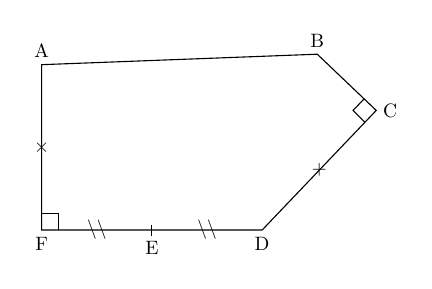
\begin{tikzpicture}[scale=0.7,every node/.style={scale=0.7}]

\draw (0,3) node[above] {A}--(5,3.19) node[above] {B}--(6.07,2.17) node[right]{C}--(4,0) node[below]{D}--(2,0)node[below=0.8mm]{E}--(0,0) node[below]{F}--cycle;
\draw (0.3,0)|-(0,0.3);
\draw (5.85,2.38) -- (5.65,2.17)--(5.86,1.96);
\draw (2,0.1)--(2,-0.1);
\draw (1,0) node {$\backslash \backslash$};
\draw (3,0) node {$\backslash \backslash$};
\draw (0,1.5) node {$\times$};
\draw (5.035,1.085) node[rotate=45] {$\times$};

\end{tikzpicture}
